
\section{Problema Desacoplado}

%->8-------------------------------------------------------------------------------------------8<-%
\begin{frame}[fragile]
  \frametitle{Problema Desacoplado}

  \begin{center}
    Se o problema fosse \[\argmin{Q,t} \fnorm{Q\blue{A} + t e\t - \red{B}},\] nós saberíamos resolvê-lo centralizando os pontos e usando o SVD!


  \[\argmin{Q} \fnorm{Q\blue{A} - \red{B}} = U V\t\text{, onde } \red{B} \blue{A}\t = U \E V\t.\]


  \[Q , t \in \argmin{Q,t} \fnorm{Q\blue{A} + t e\t - \red{B}} \Leftarrow Q = \bar{U} \bar{V}\t \text{ e } t = \red{b} - Q\blue{a}\]

  onde $\bar{\red{B}} \bar{\blue{A}}\t = \bar{U} \bar{\E} \bar{V}\t$ e $\bar{\red{B}}$ e $\bar{\blue{A}}$ são $\red{B}$ e $\blue{A}$ centralizados, $\red{b} = \dfrac{1}{n} \red{B} e$ e $\blue{a} = \dfrac{1}{n} \blue{A} e$.
  \end{center}
\end{frame}
%->8-------------------------------------------------------------------------------------------8<-%

%->8-------------------------------------------------------------------------------------------8<-%
\begin{frame}[fragile]
  \frametitle{Problema Desacoplado}
  \begin{code}
    function procrustes(X, Y)
      U, _, V = svd(Y * X')
      return U * V'
    end
  \end{code}
  \begin{code}
    function best_rigid_transf(X, Y)
      _, n = size(X)

      x = 1/n * X * ones(n)
      y = 1/n * Y * ones(n)
      Q = procrustes(X .- x, Y .- y)

      return Q, y - Q * x
    end
  \end{code}
\end{frame}
%->8-------------------------------------------------------------------------------------------8<-%

%->8-------------------------------------------------------------------------------------------8<-%
\begin{frame}[fragile]
  \frametitle{Problema Desacoplado}

  \begin{center}
    Se o problema fosse \[\argmin{P} \fnorm{\blue{A} - \red{B}P},\] saberíamos resolvê-lo usando \texttt{for}!

    \vspace{1cm}
    Verificando todas as distâncias das colunas de uma matriz para a outra e colocando o valor $1$ no índice da linha da matriz $P$ relativa ao ponto de menor distância.
  \end{center}
\end{frame}
%->8-------------------------------------------------------------------------------------------8<-%

%->8-------------------------------------------------------------------------------------------8<-%
\begin{frame}[fragile]
  \frametitle{Problema Desacoplado}
  \begin{figure}
    \centering
    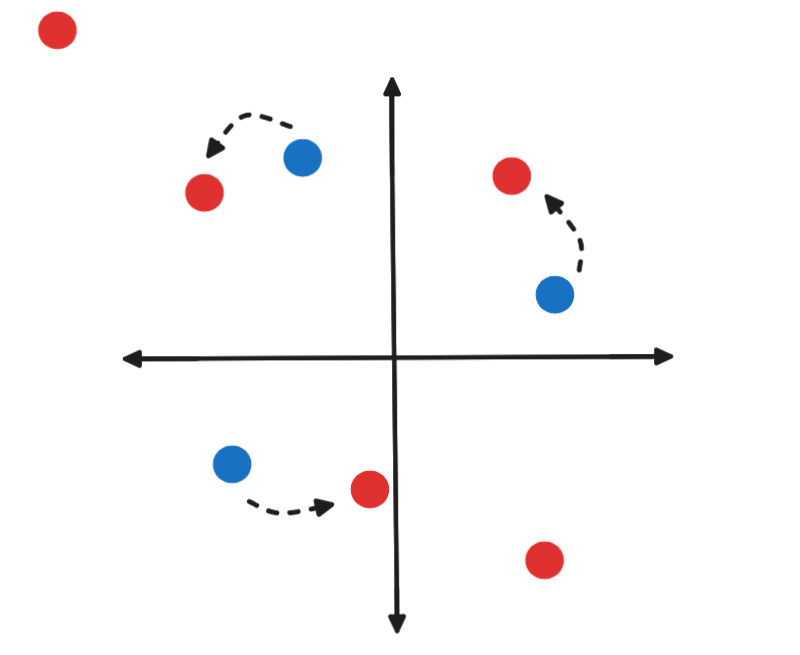
\includegraphics[width=0.75\textwidth]{best-P.png}
  \end{figure}
\end{frame}
%->8-------------------------------------------------------------------------------------------8<-%

%->8-------------------------------------------------------------------------------------------8<-%
\begin{frame}[fragile]
  \frametitle{Problema Desacoplado}
  \begin{code}
    function best_indicator(X, Y)
      nx, ny = size(X, 2), size(Y, 2)
      P = zeros(ny, nx)

      for i in 1:nx
        best_j = argmin([norm(X[:, i] - Y[:, j]) for j in 1:ny])
        P[best_j, i] = 1
      end

      return P
    end
  \end{code}
\end{frame}
%->8-------------------------------------------------------------------------------------------8<-%
